
\newpage 
\section{Embedding policy, practice and supports to advance professional, managerial and support staff careers}
\label{sec:pms}

Professional, managerial, and support staff as discussed in this section includes research support staff as well as School PMS staff.
%This section considers PMS staff in traditional academic functions but also explicitly includes staff that provide professional, managerial and support functions in a research context. The nature of whether such staff are considered “research” or “administrative” staff from the perspective of the University is complex and may be linked to historical or contractual obligations. However, many would identify as belonging to the PMS category given that their role is to support or manage research but not actively partake in the research itself. 

\subsection{Reflecting on recruitment practices in the department, answer the following:}

\instr{
\begin{prompt}
\setlength\tabcolsep{6pt} 
\begin{tabu} to \textwidth { X[8] X X }    
     \multirow{2}{=}{Recruitment to PMS posts in the department adheres to institutional policy on recruitment, which includes gender-balanced panels and training for assessors.} & \textbf{Yes} & \textbf{No}  \\
     &  \XBox & \Square  \\ 
\end{tabu}
\setlength\tabcolsep{0pt} 
\end{prompt}

If you answered ‘no’, please comment.
}


%%% KS this text should go, as no comments are necessary in response to this question.

% As previously stated, CSIT adheres to UCC’s recruitment policy, including gender diverse selection panels where feasible, and a requirement that all selection committee members undergo Equality in Recruitment training. Unfortunately, UCC does not currently maintain selection committee data for PMS posts, except in a research context. Partial records relating to selection committee composition were gathered within CSIT as per Table~\ref{tab:selectioncommittee:pms}. 
% Over a three-year period, there was a relatively even distribution in the gender of chairs. The majority of appointed candidates were male especially for the senior research PMS roles which may be attributable to a small number of applicants or few female applicants, as discussed in the next section. Most selection committees showed diversity in the gender of board members which is notable given the small number of females across all roles within the School. 

% Measures are discussed in the following section to attract greater gender diversity in applicants and to make the recruitment process as inclusive as possible. To determine if these measures are effective, it must be ensured that complete genderised data records relating to all PMS positions are available. Specifically, this should include selection committee gender composition, gender composition of applicants and those shortlisted, and appointment outcomes. As such, Action \todo{<DT/JM Data action>}, as stated in Section 1, is necessary. 

      


\begin{tabbox}{!th}
\caption[Gender composition of selection committees for PMS Appointments]{Gender composition of selection committees for PMS Appointments (2017-2020)}
\label{tab:selectioncommittee:pms}
\footnotesize 
\sisetup{
    group-digits=all,
    group-minimum-digits=4,
    group-separator = {,},
    mode=text,
    reset-text-series = false, 
    text-series-to-math = true,
    reset-text-family = false, 
    text-family-to-math = true
}
\begin{tabular}{P{2cm}
                P{6.5cm}
                C{1.3cm}
                C{1.3cm}
                !\qquad
                C{1.3cm}
                C{1.3cm}
                }
\toprule
    {Year} & 
    {Competition} & 
    \multicolumn{2}{c}{{\makecell{Chair Person}}} & 
    \multicolumn{2}{c}{{\makecell{Board Members}}} \\
    \cmidrule(l){3-4}\cmidrule(l){5-6}
    & & {F} & {M} & {F} & {M} \\
\midrule

\multicolumn{2}{l}{Administrative  (School)}\\

\midrule 
2018 & Senior Executive Assistant & 1 & 0 & 1 & 1 \\
\hdashline
2020 & Executive Assistant & 1 & 0 & 1 & 1 \\

\midrule 
\multicolumn{6}{l}{Systems Administrative  Support}\\
\midrule 

2019 & Computing Systems Engineer & 1 & 0 & 0 & 3 \\

\midrule
\multicolumn{6}{l}{Research Support}\\
\midrule

2017/18 & Systems \& HPC Lead, Insight & 1 & 0 & 2 & 4 \\

\hdashline

2018/19 & Senior Research Coordinator (EU Programme Manager), Insight & 0 & 1 & 0 & 1 \\

\cdashline{2-6}

 & Research Support Officer & * & * & * & *\\

\cdashline{2-6}

 & Senior Research Coordinator (Advance CRT Programme Manager) & 0 & 1 & 2 & 0 \\

\hdashline 

2019 /20 & Research Assistant (ADVANCE CRT) & 0 & 1 & 1 & 1  \\


\cdashline{2-6}
 & Senior Research Coordinator (CONFIRM) & 0 & 1 & 1 & 1 \\

\cdashline{2-6}

 & Research Coordinator (Insight) & 0 & 1 & 1 & 1  \\

\bottomrule
\end{tabular}
\\[2mm]
{
\footnotesize\sffamily 
* Data not available
}

\end{tabbox}




\subsection{Provide three years of data on application, shortlist, and appointment rates for recruitment by gender and grade. Where data suggests opportunity for improvement, comment and reflect. Include any other relevant information relating to recruitment processes and practice for professional, managerial and support staff in the department.}


Table~\ref{tab:pms:appointment} shows recruitment data for PMS staff. %, as gathered from partial CSIT records. 
Over a three-year period, there was a relatively even distribution of genders across those shortlisted.  
There is greater gender diversity in the applicants for the research PMS posts. However a challenge exists in attracting a gender diverse pool of applicants to the School and Systems administration posts which are mainly female and male, respectively. The systems administration group is currently all male (5 staff) and the School’s administrative group is currently all female (5 staff). A male staff member was recruited to the School’s administrative group in 2018 
but has recently moved to a research PMS role. 
%As part of the EDI survey, PMS staff were asked to reflect on the recruitment process. 
Although 12 PMS staff took the EDI survey, only 1-3 responses were received for recruitment questions. Those that answered were content with the recruitment process.

The PMS working group discussed at length causation of gender imbalance in certain roles as well as possible mechanisms to address this. 
%Approaches used by other Athena SWAN awardees that were consulted as part of the self-assessment process (Professor Ita Richardson of Lero, University of Limerick and Professor Lucy Hederman of Trinity College Dublin) were discussed. 
These included targeted recruitment strategies and making use of a gender language software to check for bias\footnote{\url{https://capd.mit.edu/resources/gender-decoder/}} in advertisements. It was agreed that the new \ac{EDI} implementation committee (EDIIC) will review the language used in advertisements to provide equitable language. This was captured in Action~\ref{action:acad:marketing} (see page \pageref{action:acad:marketing}).

Furthermore the PMS working group discussed how to convey to potential candidates the EDI friendly ethos of the School in order to attract as many female applicants as possible. It was decided to review all School materials (images and text) to convey the flexible, inclusive and collegiate nature of the School (see Action~\ref{action:materials:guidelines}). %<Kieran action review materials> in the previous section. 

Periods of leave can have a negative impact on the career of women in academia leading to gender inequalities. The working group discussed how this situation may have worsened since the Covid-19 pandemic, supported by a growing body of literature suggesting it has had a major impact on women’s employment. As such, Action~\ref{action:acad:cvgaps} (see page \pageref{action:acad:cvgaps}) 
%<Dirk action leave statements> 
was proposed to invite individuals to account for documented leave, caring responsibilities and pandemic related gaps in their CV. 
%In this way, prospective applicants can be shortlisted and assessed in a more holistic manner. 

%**** INSERT TABLE 2.3.2 HERE *** 


\begin{tabbox}{!th}
 
      
\footnotesize 
\caption{Recruitment of PMS staff by competition and gender (2017-2020)}
\label{tab:pms:appointment}
\sisetup{
    group-digits=all,
    group-minimum-digits=4,
    group-separator = {,},
    mode=text,
    reset-text-series = false, 
    text-series-to-math = true,
    reset-text-family = false, 
    text-family-to-math = true
}
\begin{tabular}{P{1.5cm}P{3.8cm}C{1.0cm}
                                C{1.0cm}
                                C{0.9cm}
                                !\qquad
                                C{1.0cm}
                                C{1.0cm}
                                C{0.9cm}
                                !\qquad
                                C{1.0cm}
                                C{1.0cm}}
\toprule
    {Year} & 
    {Competition} & 
    \multicolumn{3}{c}{{\makecell{Applicants}}} & 
    \multicolumn{3}{c}{{\makecell{Shortlisted}}} &
    \multicolumn{2}{c}{{\makecell{Appointed}}}\\
    \cmidrule(l){3-5}\cmidrule(l){6-8}\cmidrule(l){9-10} 
    & & {F} & {M} & {\%F} & {F} & {M} & {\%F} & {F} & {M}\\
\midrule

\multicolumn{2}{l}{Administrative  (School)}\\

\midrule 
2018 & Senior Executive Assistant & 6 & 1 & 86\% & 3 & 1 & 75\% & 0 & 1\\
\hdashline
2020 & Executive Assistant & 6 & 0 & 100\% & 4 & 0 & 100\% & 1 & 0\\

\midrule 
\multicolumn{8}{l}{Systems Administrative  Support}\\
\midrule 

2019 & Computing Systems Engineer & * & * & * & * & * & * & * & 1\\

\midrule
\multicolumn{8}{l}{Research Support}\\
\midrule

2017/18 & Systems \& HPC Lead, Insight & 0 & 1 & 0\% & 0 & 1 & 0\% & 0 & 1\\

\hdashline

2018/19 & Senior Research Coordinator (EU Programme Manager), Insight & 0 & 2 & 0\% & 0 & 1 & 0\% & 0 & 1\\

\cdashline{2-10}

%2018/19 
& Research Support Officer & 1 & 0 & 100\% & 1 & 0 & 100\% & 1 & 0\\

\cdashline{2-10}

%2018/19 
& Senior Research Coordinator (ADVANCE CRT Programme Manager) & \multicolumn{2}{c}{(8)} & -- & 2 & 2  & 0\% & 0 & 1 \\

%2019 /20 & Research Assistant (ADVANCE CRT) & 0 & 1 & 1 & 1 & 1 & 0 \\
\hdashline

2019/20 & Research Support Officer & 3 & 10 & 23\% & 3 & 10 & 23\% & 1 & 0\\

%\hdashline
% 2019 /20 & Senior Research Coordinator (CONFIRM) & 0 & 1 & 1 & 1 & 0 & 1\\

\cdashline{2-10}

%2019/20 
& Senior Research Coordinator (ADVANCE CRT) & 2 & 3 & 40\% & 2 & 3 & 40\% & 0 & 1\\

\cdashline{2-10}

%2019 /20 
& Research Coordinator (Insight) & 4 & 1 & 80\% & 4 & 1 & 80\% & {\makecell{Not\\filled}} & {\makecell{Not\\filled}} \\

\bottomrule
\end{tabular}
\\[2mm]
{
\footnotesize\sffamily 
* Data not available\\
(n) gender not recorded; total number n reported
}

\end{tabbox}



The working group discussions revealed a potential factor for why applicants may be discouraged to apply for research PMS positions: School PIs and a recent research PMS appointee pointed out that the documentation required from prospective applicants is not always applicable to the responsibilities of the role, such as a list of research publications. 
This could discourage potentially suitable candidates from applying. 
%In this instance, the staff member knew the post would match their skills as they had already worked in the School in another capacity and hence was aware of the role's responsibilities in practice. 
In order to prevent applicant confusion regarding what research PMS roles entail, potentially limiting the pool of applicants, Action~\ref{action:pms:matchdescription} has been proposed. 

\newcommand{\actpmsmatch}{
Ensure that advertisements for research PMS posts clearly identify the key duties / responsibilities associated with the post. 
}

\begin{actionblock}{\ksspace{}Revise PMS Application Forms Locally}{pms:matchdescription}
\actpmsmatch
\hfill{
    \hypersetup{hidelinks}
    \hyperlink{d3}{\gotoactionsymbol{}}
}
\end{actionblock}


Finally, part of Action~\ref{action:enrich:opportunities} %<Kieran action internship to female UGs> 
(see page \pageref{action:enrich:opportunities}) provides an opportunity for female undergraduate students to gain relevant work experience, includes within the School's systems administration group. 
This replicates a UCC IT services helpdesk model where some females have gone on to assume positions within UCC IT Services. This could both provide an opportunity for female undergraduates students to gain experience as well as introducing some gender diversity to the systems administration team. %, albeit on a part-time basis.  


\subsection{Reflecting on progression in your institution, answer the following:}
\instr{
\begin{prompt}
\setlength\tabcolsep{6pt}
\begin{tabu} to \textwidth { X[8] X X }
\multirow{2}{=}{Career progression opportunities for PMS staff are centrally managed by the institution (e.g. internal vacancy competitions; regrading; promotions pathway).} & \textbf{Yes} & \textbf{No}  \\
     & {\centering \XBox } & {\centering \Square}  \\ 
\end{tabu}
\setlength\tabcolsep{0pt}
\end{prompt}

If you answered ‘no’, please comment on the department’s role in career progression for professional, managerial and support staff. 
}

All administrative promotions are handled centrally within UCC. There is no automatic grade progression in place for PMS staff. 
The EDI survey and the PMS focus group indicated that most PMS staff either expressed no interest in the career progression opportunities or a strong dissatisfaction with the lack of progression opportunities due to infrequent promotion calls and quotas in place for promotion.  

% \begin{myquote}
%     ``I must look further into the promotion process down the line, if needs be. At the moment, I am quite happy in the job I'm doing.'' 
% \end{myquote}
%and
%\begin{myquote}
%    ``I am not familiar with the promotion scheme. It does not apply to my case and therefore I have never expressed interest on it.'' 
%\end{myquote}
%and
%\begin{myquote}
%    ``I think it's quite clear that this is a problem across UCC. And the unfortunate thing is, it means that UCC doesn't get the best from staff.   People that are capable of doing more are not being given the opportunity to do that, and I think that's damaging to the whole institution.''
%\end{myquote}

%Two mechanisms exist for promotion; re-grading via internal competition or achieving a promotion by an advertised open recruitment competition. 

\subsubsection{Internal vacancy competitions}
PMS staff described that the limited opportunities that do exist to progress to a more senior grade largely come through internal recruitment, requiring a move to another part of the University.  This was perceived as involving uncertainty and risk as PMS staff are largely happy working within the School: 

% \begin{myquote}
%     ``It almost seems to be a bit of an issue, really, in the university -- you have to move around to move up. So while I really like the [School] and I would love to stay here ... it's tough to know what progression there would be. You know, you might just need to move to another department that would have an opening at a higher grade down the line or something ...''
% \end{myquote}

\begin{myquote}
    ``We want to progress but [also] to remain in the School ... because, well, I'm happy here.  And in order to [be] promoted, sometimes you need to go across campus and so that puts you off a bit because, you know, your well-being and being happy [are] very important.''
\end{myquote}

% \begin{myquote}
%     ``Moving from [one] department in the university to another department ... can cause issues.  It's almost treated like you're starting a new job [with a period of] probation ... If you're looking for loans, mortgages, things like that ... It seems like a kind of short-sighted thing to just default onto people.''
% \end{myquote}

\subsubsection{Regrading}
%The first mechanism is a University-led administrative promotion scheme that offers the opportunity for administrative staff to have their posts re-graded. 
One approach to promotion for administration staff is regrading. 
PMS staff expressed a strong sentiment regarding a lack of regrading opportunities. 
Indeed, this approach had been dormant for a long period but was reconstituted in recent years to facilitate regular promotional calls on a similar frequency to academic staff (every three years). The first of these calls occurred in 2019/2020 with a total of 53 promotions available. To the best of our knowledge, no PMS staff applied for this scheme. Another call has been recently released for the 22/23 year. 

Some female PMS staff believed that interviewers  do not have first hand knowledge or understanding of applicants roles when they are applying for progression. An action was discussed, suggesting that feedback be sent to HR that staff would like a supporting statement from direct line managers to be optionally sought for input into promotions rounds or regrading. 
%Scoring should be modified to accommodate this where suitable. 
However as a similar mechanism has been made available in the recently advertised 22/23 round, this action was not progressed locally. 


\subsubsection{Promotion pathways}
A more common approach to promotion is for staff to compete in an open competition for posts, either within their School, or often outside their Unit. 
%Such posts may be advertised internally or externally in the case of senior position and research support roles. 
%In the reporting period (2017-2020), one staff member left CSIT to take up promotions elsewhere in UCC but has subsequently returned.
%It is our view that this doesn't represent promotion but rather internal recruitment.

As part of the EDI survey, PMS staff were asked to reflect on the career progression opportunities with responses summarised in Figure~\ref{fig:survey:pms:careerprogression}. Both genders agreed that promotions are free from gender bias, with the exception of one male staff member. However, importantly, 3 female and 1 male staff members noted that the pandemic had limited their promotion opportunities and 2 females and 2 males stated that it is not clear how career breaks are considered in promotion decisions. This will be addressed with Action~\ref{action:acad:cvgaps} (see page \pageref{action:acad:cvgaps}). %<Dirk action on leave statements> as defined in the <Section 2.2> and referenced in the previous sub-section. 

PMS staff did express a desire for greater training and guidance on preparing for promotion as addressed in the next Section. The lack of guidance for PMS Staff on potential pathways to advance to more senior roles through internal recruitment was identified by one participant as a significant gap.  Given the range of diverse PMS jobs available across the University, in Schools and in central administrative units, this participant felt that guidance on potential PMS career pathways within the institution would be useful, to assist staff in identifying where and how their skills and experience might be usefully redeployed and expanded. Others concurred with this view:  

%\begin{myquote}
%    ``I think because it's an admin role, if you're going up [a grade], the [variety] of jobs is pretty wide ... And the thing is, I’m not really sure, what other skills do I need to have? ... There is no clear map ...  I wish there was [guidance] there that, [e.g.] if you specialize in this area, this is where you can grow your knowledge and skills, and this is what you can apply for in the future.  .... I [wish] that there was kind of a career map -- that everybody could see ... routes.''
%\end{myquote}

Action~\ref{action:acad:cdp} (page \pageref{action:acad:cdp}) 
%<dirk bespoke training action> 
will address this via bespoke training workshops. 

% fig 2.3.1 here

\begin{figure}[!ht]
\colorbox{orangebg}{
\begin{minipage}{14.2cm}
    \caption{Staff survey responses: career progression process}
    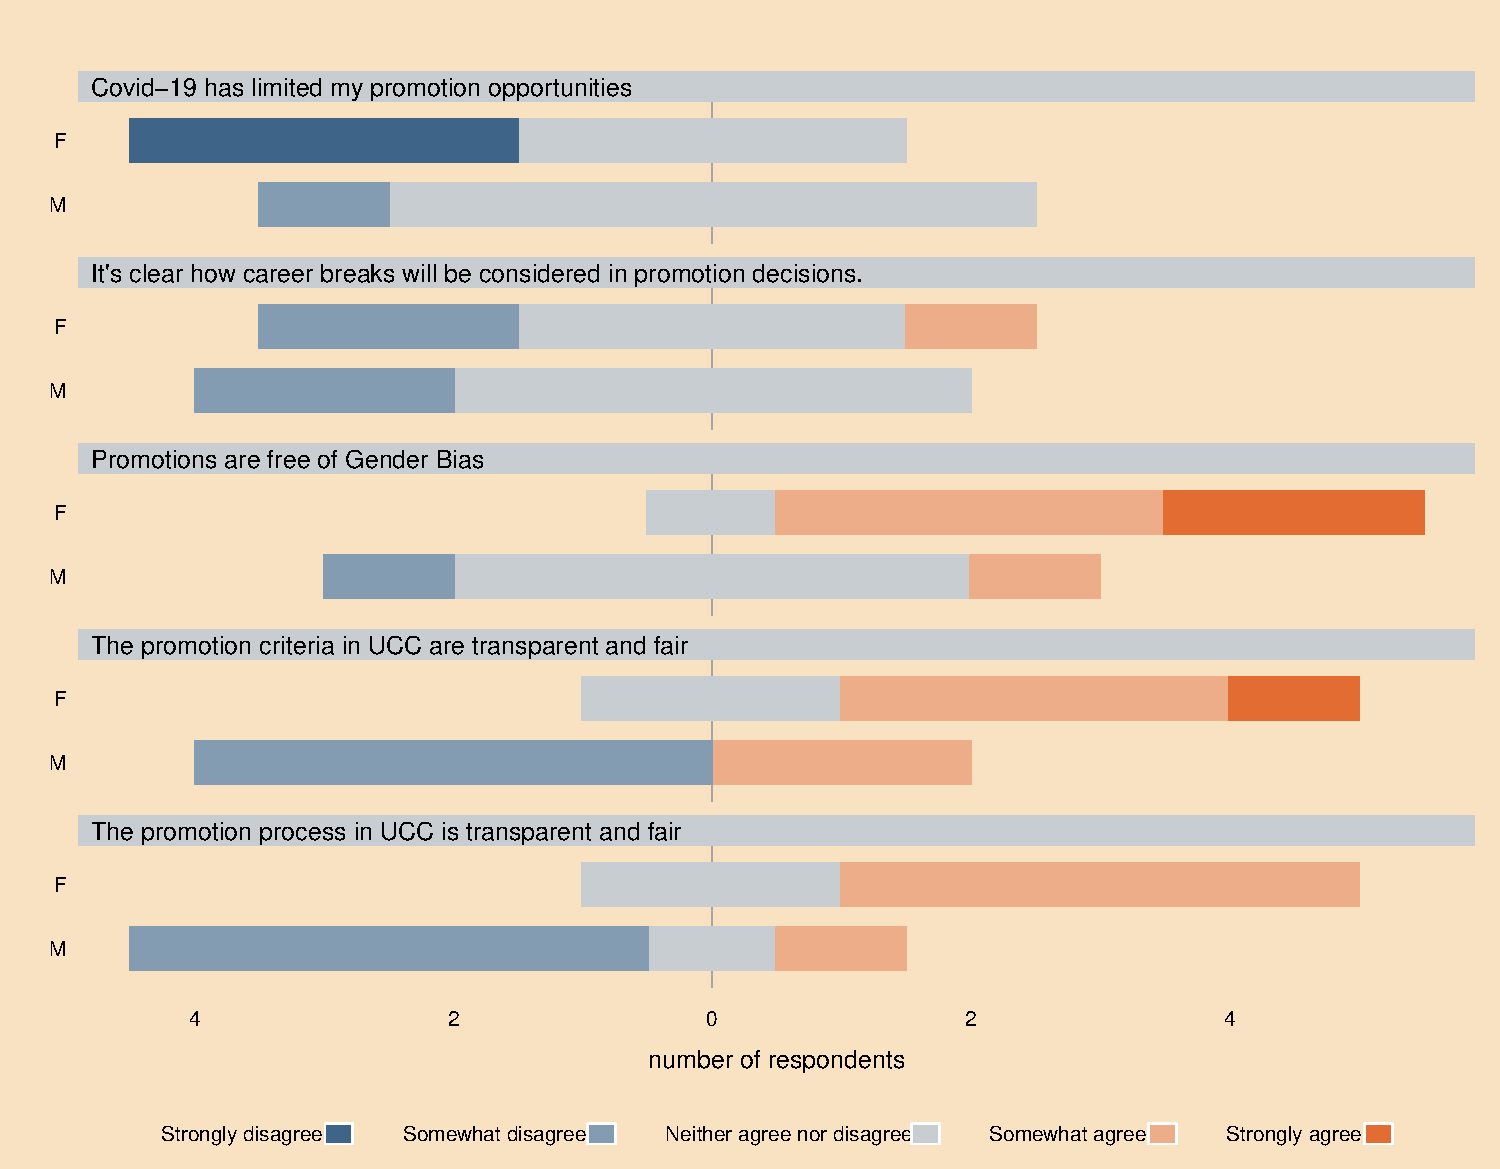
\includegraphics[trim={5mm 0 5mm 0},clip,width=5.5in]{fig/fig232.pdf}

    \label{fig:survey:pms:careerprogression}
\end{minipage}
}
\end{figure}





\subsection{Reflecting on opportunities for staff development review, answer the following:}

\instr{
\begin{prompt}
\setlength\tabcolsep{6pt} 
\begin{tabu} to \textwidth {@{} X[8] X X @{}}
     \multirow{2}{=}{The institution operates a development review process, or equivalent, for PMS staff} & \textbf{Yes} & \textbf{No}  \\
     &  \XBox & \Square  \\ 
\end{tabu}
\setlength\tabcolsep{0pt} 
\end{prompt}

If you answered `yes', comment and reflect on the implementation of this institution-level process in the department. This should include: 
\begin{itemize}
    \item data on uptake by gender;
    \item results from staff consultation presented by gender;
    \item information on any additional department-level opportunities for staff to discuss professional development, where different to above (2.\ref{sec:2e}). 
\end{itemize}
	
If you answered `no', provide detail on department-level opportunities for staff to discuss professional development, where different to above (2.e), including data on uptake by gender and results from staff consultation presented by gender. 
}


\subsubsection{Uptake of development review process by gender}
As previously stated, the University operates a Performance Development Review System (PDRS) where an Individual’s goals and objectives are set and aligned with the strategic objectives of the School and the University. The PMS \ac{PDR} structure is shown in Table~\ref{tab:pdr:structure}.
As discussed earlier (see page \pageref{action:acad:pdrs}), the CSIT has not conducted performance development reviews in recent years, but they are due to resume (see Action~\ref{action:acad:pdrs}).


\begin{tabbox}{!th}
\caption{Performance Development Review Structure in CSIT}
\label{tab:pdr:structure}
\sisetup{
    group-digits=all,
    group-minimum-digits=4,
    group-separator = {,},
    table-format=4.1,
    mode=text,
    reset-text-series = false, 
    text-series-to-math = true,
    reset-text-family = false, 
    text-family-to-math = true
}
\footnotesize   
\begin{tabular}{p{5.5cm} 
                !\quad 
                p{8.5cm}}

\toprule 
Role & Line managers who hold reviews\\
\midrule 
School PMS staff & School Manager\\
\hdashline
Systems administration PMS staff & Computing Systems Manager\\
\hdashline
Researcher PMS staff & Principal Investigators, Funded Investigators, RICU managers\\
\bottomrule 
\end{tabular}


\end{tabbox}


\subsubsection{Results from staff consultation by gender}

As part of the EDI survey, PMS staff were asked to reflect on their opportunities to discuss career progress and promotion opportunities with responses summarised in Figure~\ref{fig:survey:pms:deptsupport}. 
Female staff were content with the opportunities available with some discontent amongst male PMS staff. More notably 2 male PMS staff members noted a lack of opportunities within their roles to gain the experience require to meet promotion criteria. 

\begin{myquote}
%\myopenquote 
    ``I think as well in the School there could be more done perhaps to allow staff to gain experience or to try different things, but in their roles.''
\end{myquote}



%%*** Figure 2.3.5 HERE ***
\begin{figure}[!ht]
\colorbox{orangebg}{
\begin{minipage}{14.2cm}
    \caption{Staff survey responses: departmental support for career progression}
    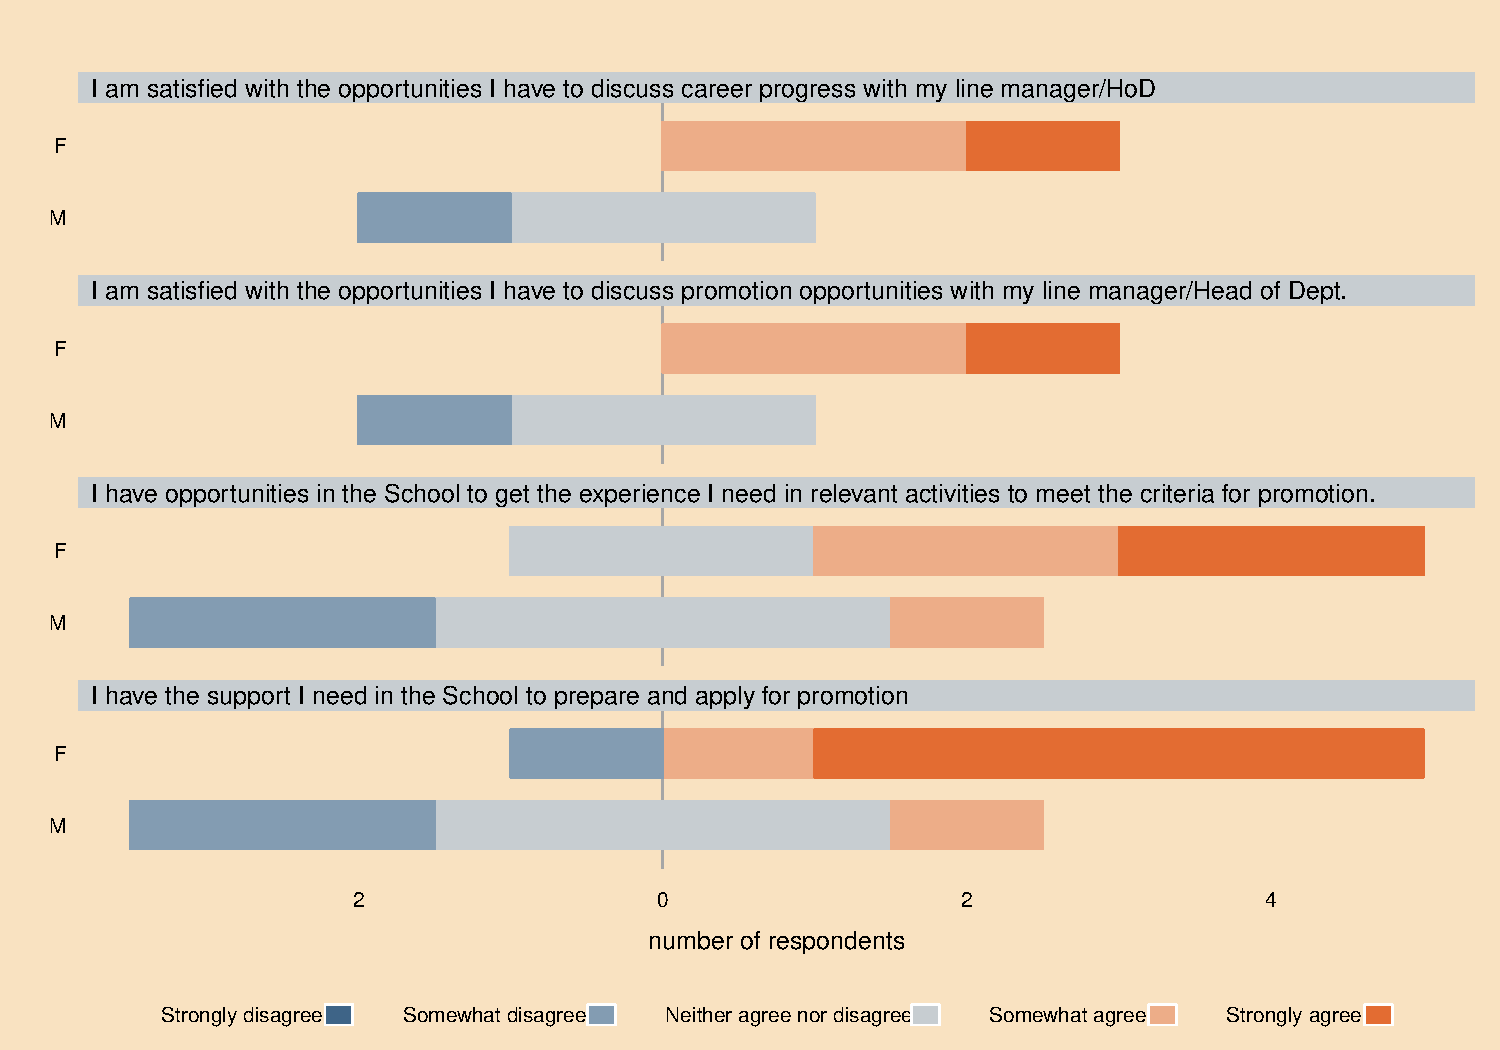
\includegraphics[width=5.5in,trim={0 0 0 0},clip]{fig/fig235.pdf}
    \label{fig:survey:pms:deptsupport}
\end{minipage}
}
\end{figure}

In the PMS focus group, participants reported that despite the absence of formal reviews, they have strong satisfaction with the opportunities available to them to discuss their career/professional development with their line managers and their support:
\begin{myquote}
    ``our line manager is very open to talking about career opportunities but obviously she has a limit. She can’t create promotion opportunities. She’s very supportive and does her best.''
\end{myquote}

\begin{myquote}
    ``There are opportunities to sit down with your line manager and get feedback. Because you know they’re very very open, the door is always open. But I suppose they’re also very restricted in what career path they can lay out for you and incentives to do well without promotional opportunities.''
\end{myquote}

To provide better support for PMS staff members 
%As it has been identified that the School could better support PMS staff members 
in their professional development, 
%by providing opportunities to gain more diverse experience, 
Action~\ref{action:pms:experience} has been proposed: % to allow PMS staff members to deputise for line managers, where appropriate. 

\newcommand{\actpmsexperience}{Provide PMS staff with regular opportunities to gain valuable professional experience to facilitate future career development.
}
\begin{actionblock}{\ksspace{}Opportunities for Professional Experience}{pms:experience}
\actpmsexperience
\hfill{
    \hypersetup{hidelinks}
    \hyperlink{d8}{\gotoactionsymbol{}}
}
\end{actionblock}


\subsubsection{Additional department-level opportunities for staff to discuss professional development}

%As highlighted in the previous section, PMS staff members have expressed their desire for greater guidance and training related to their professional and career development. Action <Dirk action on bespoke workshops> addresses this by providing multiple opportunities for a series of bespoke training sessions tailored to the needs of particular staff cohorts. 
%This follows from the delivery of a highly successful bespoke workshop delivered to the Insight centre by the UCC EDI unit. 
%Topics areas have been identified including "professional development planning using personalised training needs analysis" and "career planning". 
%Action <DT/JM staff survey action> will explicitly monitor whether these bespoke workshops are considered impactful by PMS staff. 

\subsection{Comment and reflect on department engagement with institution-level supports for PMS staff career progression as well as any department-level support available, where different from above (2.\ref{sec:2f}). This should include results from staff consultation presented by gender.}


CSIT does not operate a formal policy relating to staff training for career development and progression. Instead, an informal approach is adopted based on encouragement and raising awareness of training or progression opportunities. A wide range of training workshops are offered by the university, covering topics such as Teamwork, Leadership Potential, Leadership and Strategic Direction, People Management and Supervision, Management and Delivery of Results, and more. 
Table~\ref{tab:training:pms} shows PMS staff engagement with these workshops in the 2017-2020 time period; on balance, there is an even uptake of opportunities among males and females. 
%This information was provided by the Department of HR but is not captured locally within CSIT. It can be observed that there is an even uptake of such opportunities among genders.


\begin{tabbox}{!b}
\caption{Training uptake by PMS staff by gender}
\label{tab:training:pms}
\footnotesize 

    
\begin{tabular}{p{2cm}                
                p{9.5cm}
                !{\qquad}
                R{1cm}
                R{1cm}}
    
    \toprule 
    Year  & Course & F & M \\
    \midrule
    
    2017/18 & Mental Health Awareness for Managers & 1 & 1\\
    \cdashline{2-4}
    & Inside Out Mindfulness: Working Mindfully & 0 & 1\\
    \cdashline{2-4}
    & Lean Yellow Belt Training & 0 & 1\\
    \hdashline
    2018/19 & Senior Leadership Development: Aspiring Leaders & 0 & 1\\
    \cdashline{2-4}
    & Innovative Problem Solving & 0 & 1 \\
    \cdashline{2-4}
    & Innovative Problem Solving: Follow Up Session & 0 & 1 \\
    \cdashline{2-4}
    & Lean Yellow Belt Training & 0 & 1 \\
    \cdashline{2-4}
    & Mid Career Financial Planning & 0 & 1 \\
    \cdashline{2-4}
    & Active Listening Skills & 1 & 0 \\
    \cdashline{2-4}
    & The Effective Employee & 5 & 0 \\
    \hdashline
    2019/20 &  Engaging with People who are Angry, Anxious, or Panicked & 1 & 0\\
    \cdashline{2-4}
    & Remote Working Workshop: Employee & 0 & 1 \\
    \cdashline{2-4}
    & Remote Working Workshop: Manager  & 0 & 1 \\
    \cdashline{2-4}
    & The Effective Employee & 1 & 0 \\
    \cdashline{2-4}
    & You and Your MBTI Preferences During Covid-19 & 1 & 0 \\
    \midrule 
    Total & & 10 & 10 \\
    
\bottomrule      
         
\end{tabular}
    
\end{tabbox}

% \begin{table}[!ht]
%     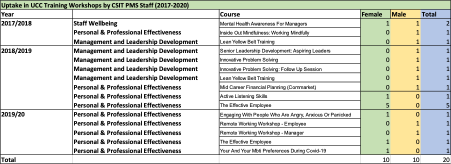
\includegraphics[width=\textwidth]{fig/table235.png}
%     \caption{Uptake in UCC training workshops by CSIT PMS staff (2017-2020) DO WE NEED THIS TABLE? CAN WE PRESENT AGGREGATE DATA?}
%     \label{tab:pms:training}
% \end{table}
% %%*** TABLE 2.3.5 HERE ***

As part of the EDI survey, PMS staff were asked to reflect on training supports for career progression with responses summarised in Figure~\ref{fig:survey:pms:trainingsupport}. 
Of the 12 PMS staff that took the EDI survey, 6 responses were received for this set of questions.  It can be observed that all females were content with the training supports available. Male PMS staff expressed some minor discontentment regarding the range of training supports and indecision/lack of opinion regarding the relevance. 

Wide and frequent dissemination of UCC training supports should be ensured, with line managers encouraging to take up relevant training opportunities to their staff members, and highlighting their relevance as appropriate (see also Action~\ref{action:acad:localsupport} on page \pageref{action:acad:localsupport}).


%%*** Figure 2.3.4 HERE ***
\begin{figure}[!ht]
\colorbox{orangebg}{
\begin{minipage}{14.2cm}
    \caption{Staff survey responses: training supports for PMS career progression}
    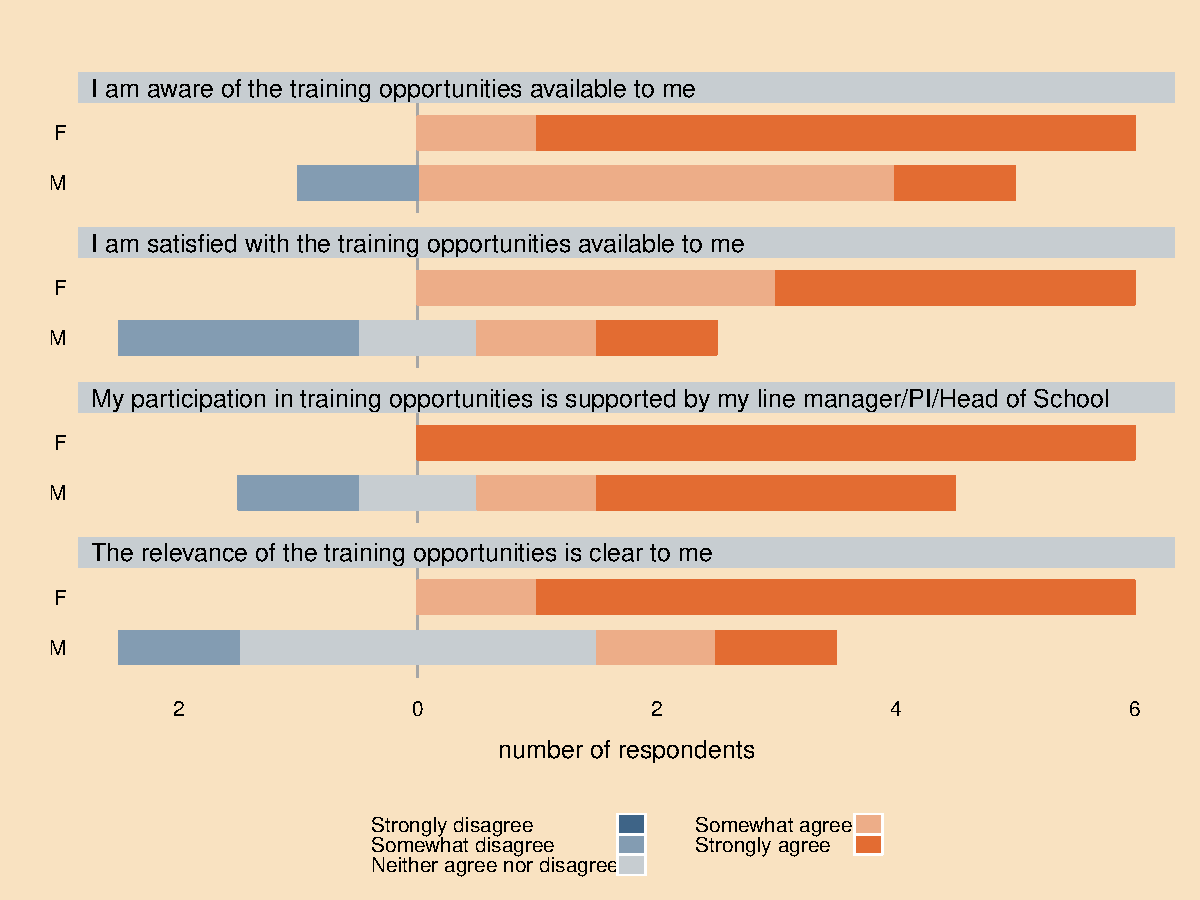
\includegraphics[width=5.5in]{fig/fig234.pdf}
    \label{fig:survey:pms:trainingsupport}
\end{minipage}
}
\end{figure}

\subsection{Comment and reflect on how workload is distributed and managed. This should include information on how the breadth of professional, managerial and support roles and responsibilities are captured in workload planning and allocation and results from staff consultation presented by gender.}

PMS staff have their workload managed by their line managers based on their role and responsibilities as per their job specification. Within the School, administrative support workload is distributed across %the following categories, allocated by the CSIT School Manager: 
several categories, including academic support, outreach and student recruitment, finance, HR, and health and safety.

% \begin{enumerate}[label=(\alph*),noitemsep]
%     \item academic support
%     \item outreach and student recruitment
%     \item finance
%     \item HR
%     \item research support
%     \item infrastructure
%     \item risk management \& control
%     \item health and safety 
%     \item school management \& strategy 
%     \item monitoring, review \& adherence
% \end{enumerate}

For systems administration staff, a similar approach is followed, with workload distributed by the Computing Systems Manager based on function (linked to the technical requirements of the School) and matched to the expertise of the systems administration staff member. %Functions are categorised as:
Functions include IT support, core systems/services, and teaching support.

% \begin{enumerate}[label=(\alph*),noitemsep]
%     \item IT Support
%     \item Core Systems
%     \item Core Services
%     \item Teaching Support
%     \item Research 
%     \item Other 
% \end{enumerate}

Research PMS staff have their workload managed by the general manager of one of the research centres (see Table~\ref{tab:researchcentres}), or by a specific Principal Investigator in the case of smaller research units. 

PMS staff were asked to reflect on their work-life balance and workload allocation (see  Figure~\ref{fig:survey:pms:worklife:female}). 
Staff were asked whether their workload is transparently allocated and whether it aligns with their career goals. Generally, female staff had no opinion or were happy, except for one staff member. Male staff members were marginally less satisfied. The pandemic did not see a significant change in these opinions. However, staff provided additional comments such as: \textit{``my workload seems to have increased as many more formal meetings,''} \textit{``If anything, the workload has increased considerably in the past 16 months''} and \textit{``Work is more intense since March 12 2020.''} 
%It was not clear that this increase in workload was gender based, but rather is attributable to the pandemic. 







% \begin{figure}[!ht]
%     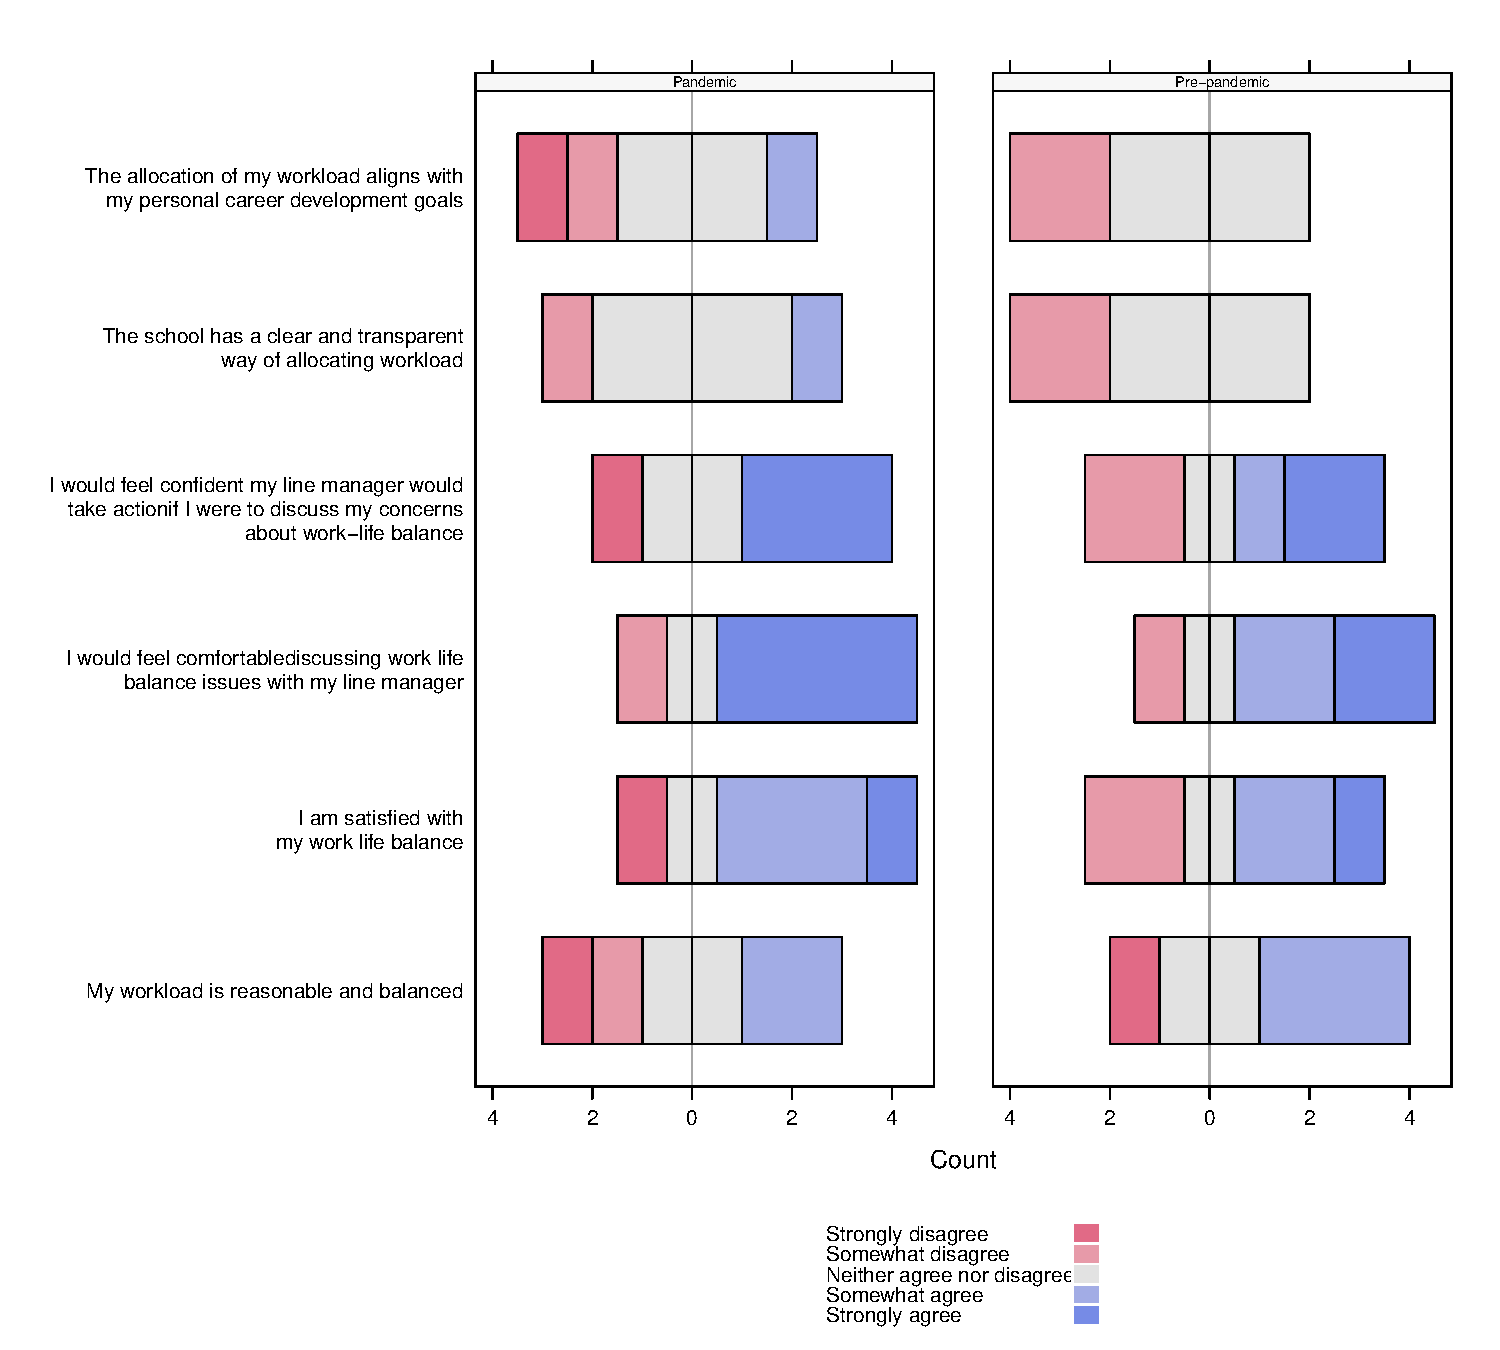
\includegraphics[width=5in]{fig/fig236-M.pdf}
%     \caption{%FIGURE IS KAPUTT - HAVE TO REGENERATE. 
%     Male staff survey responses: work/life balance and workload distribution}
%     \label{fig:survey:pms:worklife:male}
% \end{figure}

% %%*** FIG 2.3.6 HERE ***

% %%*** FIG 2.3.7 HERE ***

% \begin{figure}[!ht]
%     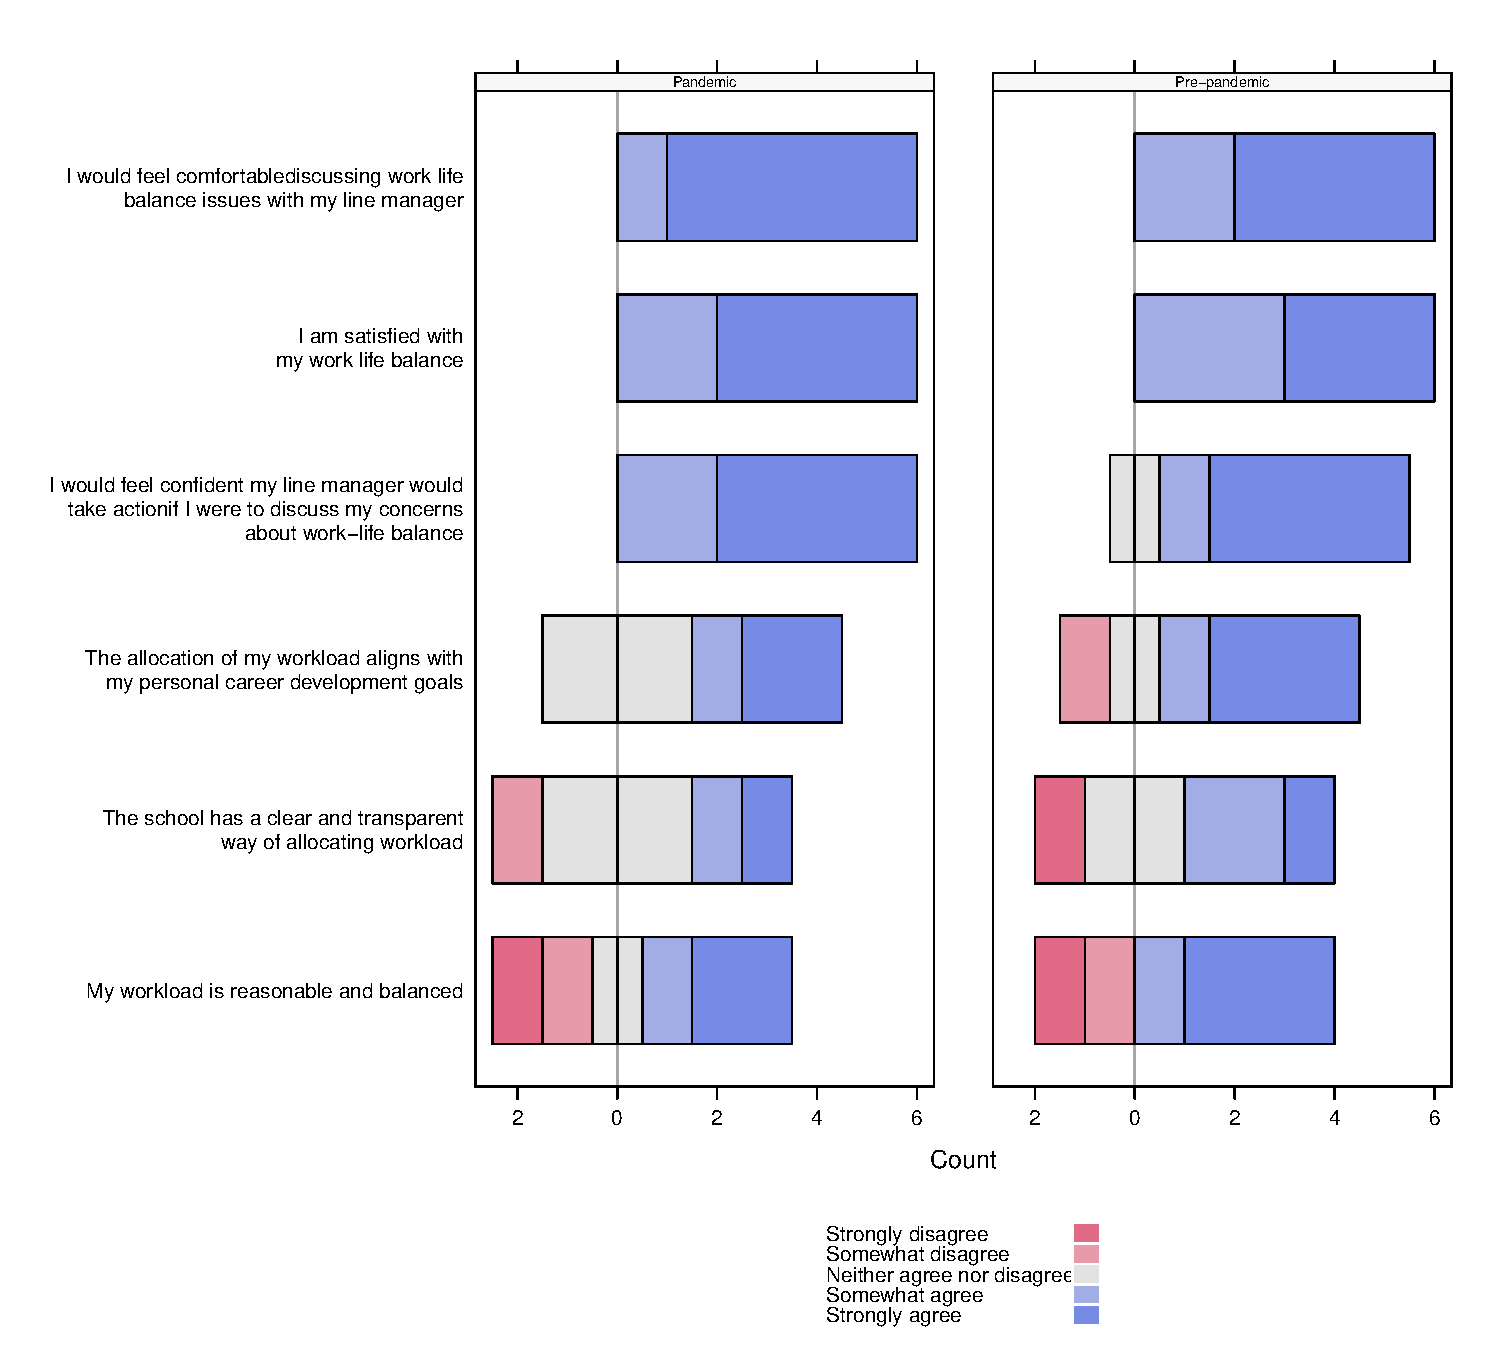
\includegraphics[width=5in]{fig/fig236-F.pdf}
%     \caption{Female staff survey responses: work/life balance and workload distribution}
%     \label{fig:survey:pms:worklife:female}
% \end{figure}



\begin{figure}[!ht]
\colorbox{orangebg}{
\begin{minipage}{14.2cm}
\caption{Work/life balance and workload distribution, before Covid-19 and during, by gender}
    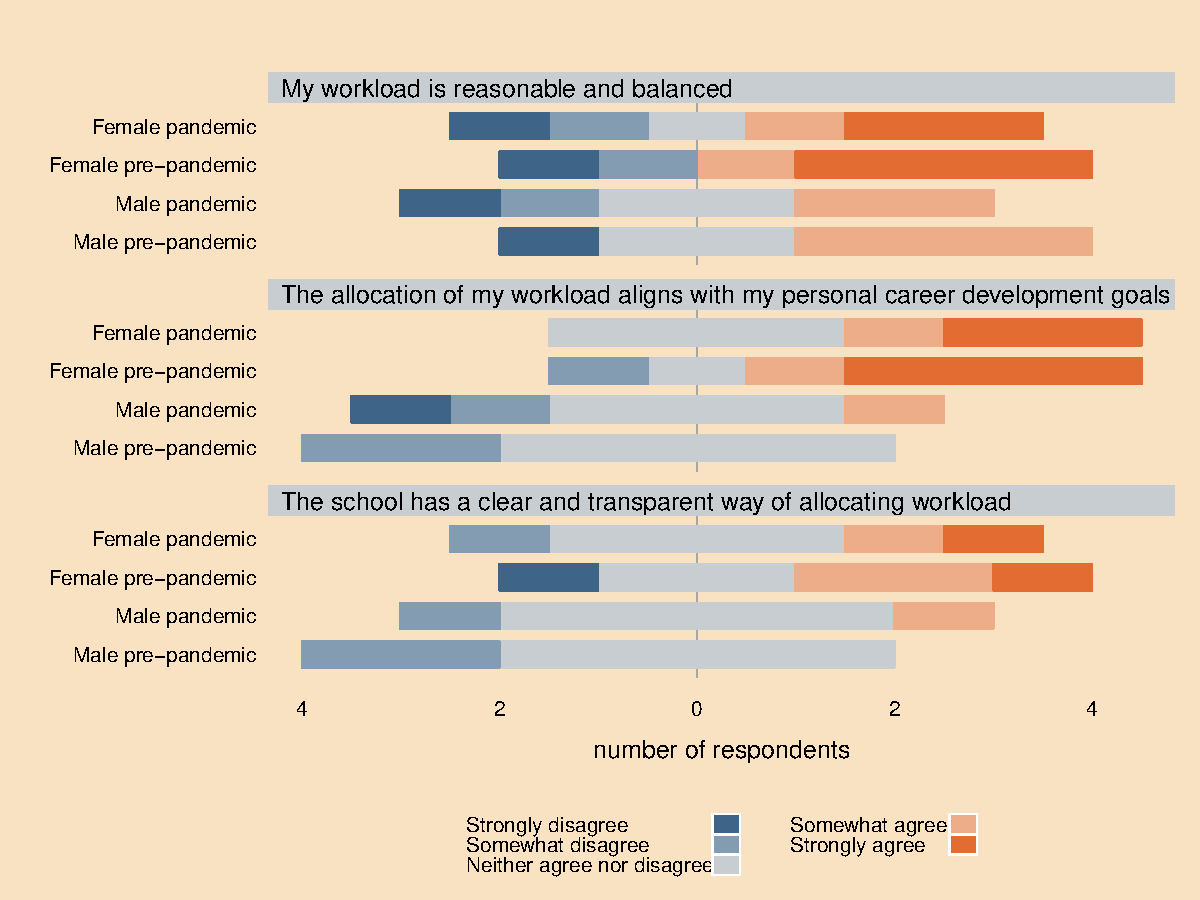
\includegraphics[width=5.5in,trim={0 0 0 0},clip]{fig/pmsworkload.pdf}
    
    \label{fig:survey:pms:worklife:female}
\end{minipage}    
}
\end{figure}



As part of the consultation, we considered the impact of the Covid-19 lockdowns on work-life balance. 
%An analysis was conducted to determine how the Covid-19 pandemic impacted work-life balance, with workload playing an attributable factor to this. 
Pre-March 2020 staff noted that \textit{``I am satisfied with my work life balance''} and \textit{``I like my job.''} 
Post March 2020 staff noted \textit{``Longer working days but greater flexibility,''} \textit{``no time wasted commuting,''} \textit{``since started working from home I find my work days to be more productive and effective.''} 
However other feedback included \textit{``The workload has gotten worse with remote working''} and \textit{``Meetings have increased significantly, and this increases stress, reduces breaks and adds to fatigue.''} 
Thus, the broad sentiments were that remote working presented benefits in terms of optimised time, flexibility and productivity, but also an increase in experienced workload and longer days.


